\documentclass[preprint,12pt]{elsarticle}
\usepackage{graphicx}
\usepackage{booktabs}
\usepackage{amsmath}
\usepackage[hidelinks]{hyperref}
\journal{Biomedical Signal Processing and Control}

\begin{document}
\begin{frontmatter}
\title{Comparative Analysis of CNN and Vision Transformer Architectures for Explainable Endometriosis Classification in Laparoscopic Images}
\author{FIRST LAST\corref{cor1}}
\affiliation{organization={DEPARTMENT, INSTITUTION}, city={CITY}, country={COUNTRY}}
\cortext[cor1]{Corresponding author: EMAIL}

\begin{abstract}
Deep learning is increasingly applied to laparoscopic images of endometriosis, and saliency maps are routinely shown alongside the predictions. Whether those maps actually fall on the lesion is rarely measured. We compared ResNet50, EfficientNet-B0 and ViT-B/16 on a balanced 746-frame subset of GLENDA under 5-fold cross-validation grouped by surgery, with confidence intervals obtained by resampling surgeries rather than frames, and we scored each model's Grad-CAM maps --- and, for the transformer, attention rollout --- against the dataset's expert lesion masks on all 373 pathology frames, using the fold models that never saw those surgeries. Classification separated the architectures only once: pooled out-of-fold AUC was 0.900 for ResNet50, 0.896 for ViT-B/16 and 0.852 for EfficientNet-B0, and after Holm correction the only difference established was ResNet50 over EfficientNet-B0 (+0.048, \emph{p} = 0.030). Explanation quality separated them clearly and in the opposite order. Against an area-matched random region and a centre-of-image prior, EfficientNet-B0 was the only model to exceed both (IoU 0.156, \emph{p} = 0.0048 against the prior), ResNet50 was indistinguishable from it (0.128 against 0.135, \emph{p} = 0.80), and ViT-B/16 was indistinguishable from chance on IoU, Pointing Game and Coverage; attention rollout performed worse still. Ranking by discrimination and ranking by explanation quality therefore disagree. We also show that grouping frames by recording segment rather than by recording --- a plausible reading of how the dataset is distributed --- introduces leakage sufficient to change which architecture appears best.
\end{abstract}

\begin{keyword}
endometriosis \sep laparoscopy \sep explainable AI \sep Grad-CAM \sep attention rollout \sep vision transformer \sep grouped cross-validation \sep medical image analysis
\end{keyword}
\end{frontmatter}

\section{Introduction}
\label{sec:intro}

Endometriosis is a chronic inflammatory condition in which tissue resembling the uterine lining grows outside the uterus --- on the peritoneum, the ovaries, and in advanced disease infiltrating deeper structures. The World Health Organization estimates that it affects about 10\% of reproductive-age women and girls worldwide, some 190 million people \cite{ref_who}. Its consequences are long-running rather than acute: chronic pelvic pain, dysmenorrhoea, dyspareunia and infertility, with the associated cost of repeated consultations, lost work and reduced quality of life \cite{ref_who,ref_e3}. It remains comparatively under-researched for a condition of that reach \cite{ref_e4}.

Diagnosis is slow. The WHO puts the average interval between symptom onset and diagnosis at four to twelve years \cite{ref_who}, a delay driven by symptoms that overlap with other pelvic conditions and by the absence of a reliable blood biomarker --- the 2022 ESHRE guideline recommends against using biomarkers for diagnosis at all \cite{ref_eshre}.

The role of surgery in that pathway has recently changed, and the change matters for where automated image analysis can help. Until recently, laparoscopy with histological confirmation was treated as the reference standard, and parts of the recent literature still describe it that way \cite{ref_e3}. The 2022 ESHRE guideline explicitly challenges that position: ultrasound or MRI is now recommended in the diagnostic work-up, and laparoscopy is reserved for patients whose imaging is negative or whose empirical treatment has failed or is unsuitable \cite{ref_eshre}. Two consequences follow. First, laparoscopy is still performed --- both for those patients and for treatment --- so what a surgeon sees through the camera still determines what is found and excised. Second, and less obviously, the patients who now reach laparoscopy are enriched for exactly the disease imaging cannot resolve: superficial peritoneal lesions, which the guideline notes a negative scan does not exclude \cite{ref_eshre}. Visual recognition during surgery therefore remains operator-dependent in precisely the cases where it is hardest, which is where decision support has something to offer.

Deep learning has been applied to this problem from several directions. Convolutional networks pretrained on natural images have been fine-tuned to classify laparoscopic frames as pathological or not \cite{ref_a2,ref_a7} and, in a preprint, \cite{ref_a5}, region-based detectors have been used to localize lesions \cite{ref_a3,ref_a6}, and work has begun on recognition during live procedures \cite{ref_a10}. Most of this work uses GLENDA, the public gynecologic laparoscopy dataset, which provides expert-annotated lesion masks alongside frame labels \cite{ref_a4}. Vision transformers have been examined for endometriosis laparoscopic video in a feasibility and ethics analysis \cite{ref_a9}, and reviews of the field summarise where the evidence currently stands \cite{ref_e1,ref_e2}.

Three problems limit what can be concluded from this literature, and they motivate what we do here.

The first is \textbf{evaluation protocol}. In the v1.5 release used here, GLENDA provides 373 annotated pathology frames against 13,438 no-pathology frames \cite{ref_glenda_web}, so accuracy on the raw set is close to meaningless: a model that never predicts the positive class scores 97\%. Studies that rebalance and studies that do not are therefore not measuring the same quantity, and reported figures cannot be compared directly. More seriously, frames extracted from one surgery are highly correlated, so any split that lets a recording contribute to both training and test data will overstate performance. This is easy to introduce accidentally: GLENDA stores no-pathology frames in per-segment folders, and treating a folder as a group --- which looks like correct grouped validation --- allows one recording onto both sides of a split.

The second is \textbf{how explanation quality is reported}. Saliency maps are commonly shown next to predictions. The one prior GLENDA study that pairs classification with explainability does score its maps against the expert masks, reporting IoU, Dice and recall \cite{ref_a1}, but it compares them against no reference level, and it reports neither the grouping unit of its cross-validation nor whether the scored maps come from models that never saw the frame's surgery. The missing reference is consequential: lesions occupy a small fraction of a frame, so a map with no spatial information still scores above zero, and a fixed centre-of-image prior can outscore a real model's map. Without such a reference, a plausible-looking overlap figure cannot be interpreted.

The third is \textbf{what a comparison between architectures can actually establish} at this sample size. Public laparoscopy data for this task amounts to a few hundred annotated frames from roughly a hundred surgeries. Differences between architectures are quantified against between-surgery variability, and treating frames as independent observations makes those differences look far more certain than they are.

This study addresses all three. Its contributions are:

\begin{enumerate}\item \textbf{A leakage-controlled benchmark on GLENDA with the grouping unit stated explicitly.} All 746 frames of a balanced subset are partitioned by surgery under 5-fold grouped cross-validation, with the partition checked programmatically and released. We also report what happens when the grouping unit is set one level too fine, because the effect on the results is large.\item \textbf{A comparison of ResNet50, EfficientNet-B0 and ViT-B/16 under one protocol, with uncertainty quantified at the level of the surgery} rather than the frame, and with raw and multiplicity-corrected \emph{p}-values reported side by side.\item \textbf{A quantitative evaluation of saliency maps against the expert lesion masks}, computed inside the cross-validation loop so that every pathology frame is scored by a model that never saw its surgery, and reported against two reference levels: an area-matched random region and a centre-of-image prior. ViT-B/16 is additionally explained with attention rollout \cite{ref_rollout}, so that its result does not depend on applying a convolution-oriented method to a transformer.\item \textbf{A direct test of whether classification performance and explanation quality order the three architectures the same way.} They do not, and that dissociation is the study's main finding.\end{enumerate}
The remainder of the paper is organised as follows. Section~\ref{sec:related} reviews related work. Section~\ref{sec:method} describes the dataset, the partitioning rule, the training protocol and the statistical and explainability analyses. Section~\ref{sec:results} reports the results. Section~\ref{sec:discussion} discusses what they do and do not support, Section~\ref{sec:limitations} sets out the limitations, and Section~\ref{sec:conclusion} concludes.

\section{Related Work}
\label{sec:related}

\subsection{Non-image approaches}

Several groups predict endometriosis without imaging at all. Symptom questionnaires analysed with standard classifiers have been proposed as a screening route that avoids surgery entirely \cite{ref_d1,ref_d2}, and transcriptomic and multi-omic signatures have been used to build predictive models of disease status \cite{ref_m3,ref_m4}. Retrospective clinical records and ultrasound findings have been mined in the same spirit \cite{ref_m1,ref_m2}. These approaches address a different point in the pathway from the one studied here: they aim to decide who should be investigated, whereas image-based work aims to support interpretation once a patient is already in surgery. The two are complementary, and the evaluation problems differ --- a symptom model is limited mainly by label quality, an image model by how its data are partitioned.

\subsection{Deep learning on laparoscopic images}

Laparoscopy is where the diagnosis is confirmed, and it is the modality closest to our task. Most published work uses transfer learning with ImageNet-pretrained convolutional networks on the GLENDA dataset \cite{ref_a4}, either classifying frames as pathological or not \cite{ref_a2} and, in a preprint, \cite{ref_a5}, or localizing lesions with region-based detectors such as Faster R-CNN and Mask R-CNN \cite{ref_a3}. Related work on comparable laparoscopic collections reports similar pipelines without naming a public dataset \cite{ref_a7}. Detector comparisons on larger private collections have also been reported \cite{ref_a6}, and early proof-of-concept work has looked at recognition during live procedures \cite{ref_a10}.

Reported figures across these studies are difficult to place side by side. The papers differ in how frames are sampled, whether the evaluated set is balanced, and --- critically --- whether frames from one surgery can appear in both training and test data. GLENDA is strongly imbalanced as distributed: the release used here contains 373 pathology frames against 13,438 no-pathology frames, a ratio of roughly 1:36, so a model that never predicts the positive class already scores 97\% accuracy. Studies that report accuracy on the imbalanced set and studies that rebalance it are therefore not measuring the same thing. Our own results (Section~\ref{sec:protocol}) show that the partitioning choice alone can reorder three architectures on a single dataset, which suggests that cross-study comparisons of headline numbers should be treated with caution.

\subsection{Other imaging modalities}

Outside laparoscopy, ultrasound and MRI have received sustained attention. Convolutional models have been applied to transvaginal ultrasound to classify endometriosis against a surgically confirmed reference standard \cite{ref_b1}, and a recent systematic review surveys that line of work \cite{ref_b4}. On MRI, deep segmentation has been used to delineate deep infiltrating lesions \cite{ref_a8}, a multi-modal pelvic MRI dataset with segmentation baselines has been released \cite{ref_c1}, and a reading-support system has been developed for clinical use \cite{ref_c2}. These modalities face a different constraint from ours: the lesion is harder to see, but acquisition is more standardised. Laparoscopy inverts that --- the lesion is directly visible, while illumination, camera and surgical technique vary from recording to recording, which is exactly the variation our error analysis traces (Section~\ref{sec:errors}).

\subsection{Transformers in surgical imaging}

Vision transformers \cite{ref_vit} have been examined for surgical video, including a feasibility analysis specific to endometriosis that also raises the ethical questions deployment would pose \cite{ref_a9}. Transformer architectures are attractive here because global self-attention can integrate evidence spread across a frame, which is plausibly useful when lesion appearance depends on surrounding tissue. That same property, however, complicates explanation: there is no convolutional feature map on which a class-activation method naturally operates, and attention weights are not by themselves an attribution. Attention rollout \cite{ref_rollout} addresses this by propagating attention through the residual stream, and we evaluate it alongside Grad-CAM rather than assuming either is adequate.

\subsection{Explainability in medical imaging}

Grad-CAM \cite{ref_gradcam} is the most widely used visual explanation in this literature, with LIME \cite{ref_lime} and SHAP \cite{ref_shap} serving similar roles for tabular and model-agnostic settings. Surveys of explainable medical imaging stress transparency and clinician trust \cite{ref_x4}, and a recent meta-analysis argues that post-hoc maps must be validated rather than displayed, reporting poor fidelity and stability for SHAP, LIME and Grad-CAM \cite{ref_x5}, and the one prior GLENDA study that combines classification with explainability \cite{ref_a1} does score its maps against the expert masks, reporting IoU, Dice and recall. What is essentially absent from this literature is any comparison of those overlap figures against a chance level. Without such a reference an IoU figure cannot be interpreted: when lesions occupy a small fraction of the frame, a map that carries no spatial information still scores above zero, and a fixed centre-of-image prior can score higher than a model's map. Section~\ref{sec:explanation} reports both references, and one of our models turns out not to exceed the simpler of them.

\subsection{What is missing}

Three gaps follow from the above, and they define what this study contributes.

First, \textbf{comparisons between CNN and transformer families are made under protocols that differ between papers, and the grouping unit is seldom stated}. A prior GLENDA study does compare four architectures under one 5-fold protocol \cite{ref_a1}; what it does not report is how frames were grouped, which decides whether the estimate is honest. We state the grouping unit, verify it programmatically, and quantify uncertainty at the level of the surgery rather than the frame.

Second, \textbf{explanation quality is reported qualitatively or not at all}. We measure the agreement between each model's saliency map and the expert lesion masks that GLENDA provides, on every pathology frame, using out-of-fold models --- and we measure it against both a chance level and a centre-of-image baseline, so that the numbers can be read.

Third, \textbf{leakage at the level of the surgery is easy to introduce and seldom documented}, though a recent detector study does address it directly \cite{ref_a6}. GLENDA distributes no-pathology frames in per-segment folders, and treating a folder as a group --- which looks like correct grouped validation --- allows one recording to contribute frames to both sides of a split. We report what that does to the results on this dataset, because the effect is large enough to change which architecture appears best.

\section{Methodology}
\label{sec:method}

\subsection{Dataset}

We use GLENDA v1.5 \cite{ref_a4}, a public dataset of frames extracted from gynecologic laparoscopy recordings. The v1.5 release contains 373 frames showing endometriosis, each with a pixel-level lesion mask drawn by medical experts, and 13,438 frames from recordings with no visible pathology \cite{ref_glenda_web}. The data are de-identified and publicly released under a CC BY-NC licence, so no additional ethical approval was required.

The raw class ratio is approximately 1:36. Reporting accuracy on such a split is uninformative, since a model that never predicts the positive class already scores 97\%. We therefore construct a balanced subset: all 373 pathology frames, and 373 no-pathology frames drawn \textbf{round-robin across the 27 no-pathology segment folders}, which correspond to 20 distinct recordings once the segment suffix is stripped, so that no single recording dominates and consecutive, near-duplicate frames are avoided. Sampling uses a fixed seed (42) and is reproduced by the script released with this work.

\subsection{Grouping and partitioning}

The unit that must not be split is the surgery, not the frame. Frames from one recording share a patient, a camera, an illumination setting and often the same lesion, so allowing them into both training and test sets would let a model recognise the recording rather than the pathology, and would inflate every reported metric. Group identity is read from the filenames: pathology frames carry a case identifier (\texttt{c\_<id>}), and no-pathology frames carry a recording-and-segment identifier. GLENDA stores no-pathology frames in per-segment folders, so one recording can appear under several folder names; the segment suffix is stripped, since two segments of one recording are the same surgery. The balanced subset comprises 746 frames from 122 surgeries: 102 pathology cases and 20 no-pathology recordings.

Partitioning uses \texttt{StratifiedGroupKFold} with five folds, which keeps whole groups together while balancing the class ratio as far as the group sizes allow. Within each fold, the training portion is split again, group-wise, to provide a validation set for early stopping; the fold's test portion is never used for model selection. Every partition is checked programmatically: no group may appear in more than one of train, validation and test, and the five test portions must tile the dataset exactly once. Because groups are indivisible, fold composition is not uniform --- test portions contain 125 to 179 frames and pathology prevalence ranges from 37.8\% to 66.4\% --- and this is accounted for in the choice of evaluation metric below.

A preliminary experiment used a single case-wise 70/15/15 split (528 train, 111 validation, 107 test frames) built by the same grouping rule. We report it in Section~\ref{sec:protocol} as a comparison, not as a result.

\subsection{Models and training}

Three ImageNet-pretrained architectures are compared, covering two convolutional designs of very different capacity and one transformer:

\begin{itemize}\item \textbf{ResNet50} \cite{ref_resnet} (\texttt{IMAGENET1K\_V2} weights), 25.6M parameters\item \textbf{EfficientNet-B0} \cite{ref_efficientnet} (\texttt{IMAGENET1K\_V1}), 5.3M parameters\item \textbf{ViT-B/16} \cite{ref_vit} (\texttt{IMAGENET1K\_V1}), 86M parameters\end{itemize}
Parameter counts are those reported by torchvision.

In each case the classification head is replaced by a two-unit linear layer and the whole network is fine-tuned; no layers are frozen. Frames are resized to 224$\times$224 and normalised with ImageNet statistics. Training augmentation is deliberately mild --- horizontal flip, rotation up to $\pm$15$^{\circ}$, and brightness and contrast jitter of 0.2 --- because laparoscopic frames have no canonical orientation but do carry diagnostic colour information. Validation and test frames receive no augmentation.

All models are trained with Adam, batch size 32, for at most 30 epochs, with early stopping when validation ROC-AUC has not improved for six epochs; the weights of the best validation epoch are restored before testing. The learning rate is 1e-4 for the convolutional networks and 2e-5 for ViT-B/16, the transformer requiring the smaller step to fine-tune stably on a dataset of this size. Identical settings, seeds and schedules are used in all 15 fits (3 architectures $\times$ 5 folds). Seeds are fixed at 42 and offset by the fold index, and cuDNN is restricted to deterministic algorithms so that a re-run reproduces the reported numbers. Training ran on a single Tesla T4 GPU in Google Colab.

\subsection{Evaluation}

Endometriosis is the positive class throughout. We report accuracy, precision, recall, F1 and ROC-AUC. Results are summarised in two ways: as the mean and standard deviation of the five fold-level values, and as \textbf{pooled out-of-fold} metrics, in which the predictions of all five folds are concatenated and each metric is computed once over the resulting 746 frames. Pooling is possible because every frame is predicted exactly once, by the model that never saw its surgery; it yields one estimate over the whole dataset instead of an average of five estimates over fifths of it.

The \textbf{pooled estimate is pre-specified as the primary result}, and every inferential comparison is made on it; fold means and standard deviations describe between-fold variability and are not a second estimate of the same quantity. Pooling requires the five fold models' scores to be comparable on one scale, which we do not verify directly; the two summaries are therefore reported side by side rather than treated as interchangeable.

ROC-AUC is treated as the primary metric because it does not depend on the fixed 0.5 threshold, so changes in fold prevalence do not move it the way they move accuracy and precision. Fold-level AUC still varies with case mix, and we do not claim it is invariant across folds.

\subsection{Statistical analysis}

All intervals are 95\% percentile bootstrap intervals from 10,000 resamples, and all tests are two-sided. \textbf{The resampling unit is the surgery, not the frame.} Frames within a recording are correlated, so resampling frames would count repeated views of one case as independent evidence; since the inference of interest is to new surgeries, whole groups are resampled, with pathology and no-pathology groups drawn separately so that both classes are present in every resample. For reference, we also report how much narrower the frame-level intervals would have been.

Architectures are compared pairwise on the pooled out-of-fold predictions with two paired bootstrap tests --- of the AUC difference and of the accuracy difference --- in which both models are evaluated on the same resampled surgeries. McNemar's exact test on discordant frames is reported alongside them because the counts are informative, but it assumes independent pairs and therefore ignores the clustering; we label it frame-level and do not use it to support claims. \emph{p}-values are Holm-corrected within each pre-specified family, and raw values are reported too, since an uncorrected interval excluding zero can sit beside a corrected \emph{p} above 0.05. The families are: the three pairwise classification comparisons; the six pairwise localization comparisons; the eight localization-versus-reference comparisons; and the eight comparisons of Pointing Game and Coverage against chance.

Training used cross-entropy loss without class weighting --- the subset is balanced --- and Adam with its torchvision defaults apart from the learning rate; scores are the softmax probability of the positive class. The validation set inside each fold is drawn with the same \texttt{StratifiedGroupKFold} splitter and seed as the outer loop, taking the first split of the training portion, which yields 92 to 124 frames depending on the fold.

\subsection{Explainability}

Classification metrics say whether a model is right; they say nothing about whether it is right for the right reason. GLENDA's expert masks allow the second question to be asked quantitatively, by comparing each model's saliency map with the annotated lesion.

Grad-CAM \cite{ref_gradcam} is computed at the last convolutional stage of each CNN (\texttt{layer4[-1]} for ResNet50, \texttt{features[-1]} for EfficientNet-B0). For ViT-B/16 the last encoder block's first layer-norm is used, with token activations reshaped into a 14$\times$14 grid. Grad-CAM was designed for convolutional feature maps, so ViT-B/16 is additionally explained with \textbf{attention rollout} \cite{ref_rollout}, the transformer-native alternative: an identity matrix is added to each layer's head-averaged attention to account for the residual connection, each row is renormalised, the layers are multiplied together, and the class token's row of the product gives each patch's contribution. Both maps are normalised to [0, 1] and upsampled to 224$\times$224.

Maps are scored against the binarised mask on three measures:

\begin{itemize}\item \textbf{IoU} between the mask and the region where the map exceeds 0.5\item \textbf{Pointing Game}: whether the map's single highest point lies inside the mask\item \textbf{Coverage}: the share of the map's total intensity that falls inside the mask\end{itemize}
These numbers are meaningless without a reference, because lesions occupy only 7.20\% of a frame on average. An uninformative map scores the mask's area fraction on both Pointing Game and Coverage. IoU needs more care, since it grows with the size of the region a method claims: each method is therefore compared against a random region of \textbf{exactly the area that method claimed}. Writing \emph{p} for the fraction of the frame a method's thresholded map covers and \emph{m} for the fraction the mask covers, a region of area \emph{p} placed independently of the mask overlaps it by \emph{pm} in expectation, so its expected IoU is \emph{pm}/(\emph{p}+\emph{m}$-$\emph{pm}). The construction assumed is a spatially uniform random region, not a connected blob; we confirmed the closed form by thresholding uniform noise at the quantile that reproduces area \emph{p} and measuring the IoU directly: over 25 frames at 400 random placements each, the analytic floor averages 0.0330 and the simulated floor 0.0330 (released as \texttt{results/iou\_floor\_validation.csv}). As a second, competing baseline we score a centred Gaussian ($\sigma$ = 0.25$\times$224), min-max normalised to [0, 1] and thresholded at the same 0.5 as every method, so its claimed area follows from the same rule rather than being matched to anything. It encodes the prior that lesions tend to appear mid-frame without looking at the image at all. Exceeding it is additional evidence for lesion-specific localization; failing to exceed it means a method has not been shown to do more than that prior.

Saliency maps are computed inside the cross-validation loop, immediately after each fold's model is evaluated and before it is discarded, so that all 373 pathology frames are scored by the same models that produced the classification results, each on data from surgeries it never saw.

\subsection{Reproducibility}

The dataset-construction script, the training and evaluation notebook, the split manifest, the per-image predictions and saliency scores, and every analysis and figure script are released at \texttt{github.com/Mozahid-DIU/Endometriosis}. Each run records a hash of its frame-to-fold assignment, so results computed under different groupings cannot be combined by accident. Seeds are fixed and cuDNN is restricted to deterministic algorithms, which makes a re-run reproducible \textbf{within the tested environment} (Google Colab, Tesla T4, PyTorch 2.x); we do not claim bitwise reproducibility on other hardware or library versions.

\section{Results}
\label{sec:results}

Throughout, endometriosis is the positive class and every test is two-sided. Confidence intervals are 95\% percentile bootstrap intervals from 10,000 resamples in which \textbf{whole surgeries, not individual frames, are the resampling unit}; frames from one surgery share a patient, a camera and an illumination setting, so resampling frames would treat repeated views of one case as independent evidence.

The \textbf{pooled out-of-fold estimate is the primary result}: every frame is predicted once, by the model that never saw its surgery, and all inferential comparisons are made on those predictions. Fold means and standard deviations are reported as a description of between-fold variability, not as a second estimate of the same quantity; the two are different estimands and are not interchangeable.

Intervals are per-comparison and uncorrected, while \emph{p}-values are Holm-corrected within each pre-specified family of tests. Both raw and corrected \emph{p}-values are given, because an uncorrected interval that excludes zero can accompany a corrected \emph{p} above 0.05, and the two are then easy to misread as contradictory. The families are: the three pairwise classification comparisons; the six pairwise localization comparisons; the eight comparisons of localization against a reference level; and the eight comparisons of Pointing Game and Coverage against chance.

\subsection{Classification performance}
\label{sec:classification}

Table~\ref{tab:1} reports the three architectures under 5-fold grouped cross-validation, in two views of the same predictions. The upper block averages each metric over the five folds. The lower block pools the out-of-fold predictions and computes each metric once over the resulting 746 frames, each scored by the one model that never saw its surgery.

\begin{table}[t]
\centering
\caption{Classification performance under 5-fold grouped cross-validation.}
\label{tab:1}
\small
\begin{tabular}{lccccc}
\toprule
 & Accuracy & Precision & Recall & F1 & ROC-AUC \\
\midrule
\addlinespace
\multicolumn{6}{l}{\emph{Mean $\pm$ SD over folds}} \\
ResNet50 & 0.823 $\pm$ 0.098 & 0.791 $\pm$ 0.151 & 0.855 $\pm$ 0.132 & 0.815 $\pm$ 0.121 & 0.903 $\pm$ 0.082 \\
EfficientNet-B0 & 0.769 $\pm$ 0.113 & 0.722 $\pm$ 0.183 & \textbf{0.876 $\pm$ 0.097} & 0.783 $\pm$ 0.126 & 0.884 $\pm$ 0.110 \\
ViT-B/16 & \textbf{0.830 $\pm$ 0.092} & \textbf{0.821 $\pm$ 0.177} & 0.859 $\pm$ 0.060 & \textbf{0.829 $\pm$ 0.101} & \textbf{0.925 $\pm$ 0.052} \\
\addlinespace
\multicolumn{6}{l}{\emph{Pooled out-of-fold (n = 746)}} \\
ResNet50 & 0.812 & 0.786 & 0.858 & 0.821 & \textbf{0.900 [0.854--0.939]} \\
EfficientNet-B0 & 0.761 & 0.712 & \textbf{0.877} & 0.786 & 0.852 [0.776--0.916] \\
ViT-B/16 & \textbf{0.827} & \textbf{0.810} & 0.855 & \textbf{0.832} & 0.896 [0.832--0.944] \\
\bottomrule
\end{tabular}
\end{table}

The pooled ROC curves are shown in Fig.~\ref{fig:roc}.

All three models recall endometriosis frames at a similar rate (0.855--0.877) and differ mainly in how many normal frames they call positive. The pooled confusion counts (Fig.~\ref{fig:confusion}), out of 373 frames per class, are: ResNet50 TP 320, FN 53, FP 87, TN 286; EfficientNet-B0 TP 327, FN 46, FP 132, TN 241; ViT-B/16 TP 319, FN 54, FP 75, TN 298.

Threshold-dependent metrics vary more across folds than ROC-AUC does. Fold prevalence is a likely contributor --- because whole surgeries are kept together, the share of pathology frames in a fold ranges from 37.8\% to 66.4\% (Fig.~\ref{fig:folds}), which moves where a fixed 0.5 threshold sits on the score distribution. Fold-level AUC also varies (0.751--0.989 across all fits), so prevalence is not the only source of variation. ROC-AUC is used as the primary metric because it is threshold-free; accuracy is reported for completeness and is not compared across folds.

Because the evaluation set is balanced 1:1 while the source data are approximately 1:36, the precision and accuracy values above describe behaviour on this balanced set only. They should not be read as the predictive values a deployed model would achieve at the prevalence of unselected laparoscopy frames.

\subsection{Do the architectures differ?}
\label{sec:differ}

Table~\ref{tab:2} tests each pair on the pooled out-of-fold predictions. Two paired tests are reported. The AUC difference and the accuracy difference both resample the same surgeries for both models, so the two models always see identical data in every resample. McNemar's exact test is also given because the discordant counts are informative, but it treats each discordant \emph{frame} as an independent pair and so ignores the clustering the other tests correct for; its \emph{p}-values are reported as frame-level and are not used to support any claim.

\begin{table}[t]
\centering
\caption{Pairwise comparison on the pooled out-of-fold predictions. Intervals and the first two \emph{p}-columns use surgery-level resampling; Holm correction is applied within the family of three comparisons.}
\label{tab:2}
\small
\begin{tabular}{lccccc}
\toprule
Comparison (A vs B) & $\Delta$AUC (A $-$ B) [95\% CI] & \emph{p} raw / Holm & $\Delta$Accuracy [95\% CI] & \emph{p} raw / Holm & Discordant frames (A/B), McNemar \emph{p} (frame-level) \\
\midrule
ResNet50 vs EfficientNet-B0 & \textbf{+0.048 [+0.010, +0.095]} & 0.010 / \textbf{0.030} & +0.051 [$-$0.001, +0.103] & 0.058 / 0.126 & 84 / 46, 0.0011 \\
ResNet50 vs ViT-B/16 & +0.004 [$-$0.040, +0.053] & 0.87 / 0.87 & $-$0.015 [$-$0.072, +0.044] & 0.62 / 0.62 & 58 / 69, 0.38 \\
EfficientNet-B0 vs ViT-B/16 & $-$0.044 [$-$0.087, $-$0.004] & 0.029 / 0.058 & $-$0.066 [$-$0.134, $-$0.003] & 0.042 / 0.126 & 50 / 99, 0.00007 \\
\bottomrule
\end{tabular}
\end{table}

One comparison survives correction: ResNet50 discriminates better than EfficientNet-B0, by 0.048 AUC (Holm \emph{p} = 0.030). For ResNet50 against ViT-B/16 there is no evidence of a difference on either test. For EfficientNet-B0 against ViT-B/16 the point estimates favour ViT-B/16 on both measures and both uncorrected intervals exclude zero, but neither survives correction (\emph{p} = 0.058 and 0.126); this comparison is therefore inconclusive rather than null.

The contrast between the two accuracy-based tests is worth stating plainly. On discordant frames, ViT-B/16 is correct on 99 that EfficientNet-B0 gets wrong against 50 the other way, which a frame-level McNemar test calls decisive (\emph{p} = 7 $\times$ $10^{-5}$). Resampling surgeries instead of frames turns the same data into \emph{p} = 0.042, and 0.126 after Holm correction within the family of three. Those 149 discordant frames fall across 46 surgeries, five of which hold 46\% of them, so counting each frame as independent evidence overstates what the data support; we report the surgery-level result.

Taken together, this evaluation can establish only that ResNet50 outperforms EfficientNet-B0 on AUC. It does not establish an ordering among the three architectures, and with 122 surgeries it was unlikely to.

\subsection{Sensitivity to the protocol}
\label{sec:protocol}

The ordering of the three models is not stable across evaluation protocols. A single case-wise held-out split of 107 frames --- the protocol common in this literature --- ranked them ResNet50 (AUC 0.915), ViT-B/16 (0.860), EfficientNet-B0 (0.833). Grouped cross-validation gives ResNet50 0.900, ViT-B/16 0.896 and EfficientNet-B0 0.852 pooled: ViT-B/16 moves from clearly second to indistinguishable from first, and the apparent 0.08 gap between ResNet50 and EfficientNet-B0 narrows to 0.048. Fig.~\ref{fig:cvauc} places the single-split value beside the five fold-level values for each model; ViT-B/16's single-split estimate falls below all five of its folds.

A further ordering change arises from the grouping rule itself. GLENDA stores no-pathology frames in per-segment folders, and an earlier version of this analysis treated each folder as a group. Six of the twenty no-pathology recordings were thereby split into two or three groups, together accounting for 178 of the 373 no-pathology frames, and four of those six ended up with segments on both sides of a split. Under that grouping EfficientNet-B0 reached a pooled AUC of 0.913, the highest of the three; with the recording treated as one surgery it falls to 0.852 and is the lowest. We report the corrected grouping throughout and release the segment-grouped predictions alongside it, so that the size of the effect can be checked.

Taken together, the single split and the surgery-grouped cross-validation produce the same rank order, while the segment-grouped run reverses it, moving EfficientNet-B0 from last to first. We draw a claim about this dataset rather than about the literature: here, the ranking was more sensitive to the grouping rule than to the choice of architecture, which is a reason to state that rule explicitly and to prefer repeated evaluation over a single split at this sample size.

\subsection{Explanation quality}
\label{sec:explanation}

Saliency maps were scored inside the cross-validation loop, so all 373 pathology frames (from 102 surgeries) are covered by the fold model that never saw their surgery. Grad-CAM is computed for all three architectures and ViT-B/16 is additionally explained with attention rollout, the transformer-native method.

Lesions occupy 7.20\% of a frame on average (range 0.17--57.39\%), so a map carrying no spatial information scores 0.072 on Pointing Game and Coverage by construction. For IoU, which grows with the size of the region a method claims, each method is compared against a random region of exactly the area it claimed. A centred Gaussian, normalised and thresholded exactly as a saliency map is, provides a competing baseline: it encodes the prior that lesions tend to lie mid-frame without looking at the image at all, and scores IoU 0.135, Pointing Game 0.274 and Coverage 0.119.

Fig.~\ref{fig:localization} plots these values against the two reference levels.

\begin{table}[t]
\centering
\caption{Localization against the expert masks (373 out-of-fold frames, 102 surgeries), with 95\% surgery-level intervals.}
\label{tab:3}
\small
\begin{tabular}{lccc}
\toprule
 & IoU & Pointing Game & Coverage \\
\midrule
EfficientNet-B0 & \textbf{0.156 [0.133--0.180]} & \textbf{0.287 [0.233--0.347]} & 0.153 [0.128--0.181] \\
ResNet50 & 0.128 [0.111--0.147] & 0.271 [0.221--0.324] & \textbf{0.168 [0.139--0.200]} \\
ViT-B/16, Grad-CAM & 0.039 [0.033--0.047] & 0.078 [0.052--0.105] & 0.070 [0.058--0.084] \\
ViT-B/16, attention rollout & 0.014 [0.010--0.019] & 0.054 [0.030--0.082] & 0.064 [0.051--0.078] \\
\emph{Centred Gaussian baseline} & \emph{0.135} & \emph{0.274} & \emph{0.119} \\
\emph{Map with no spatial information} & \emph{area-matched} & \emph{0.072} & \emph{0.072} \\
\bottomrule
\end{tabular}
\end{table}

Unlike the classification comparisons, the differences between methods are large relative to their uncertainty. All six pairwise IoU differences are significant after Holm correction within that family; Table~\ref{tab:4a} lists four of them, the two omitted being ResNet50 and EfficientNet-B0 against attention rollout (+0.114 and +0.142, both \emph{p} = 0.0006): EfficientNet-B0 exceeds ResNet50 by 0.029 (\emph{p} = 0.004), both CNNs exceed ViT-B/16 by 0.088 and 0.117 (\emph{p} = 0.0006), and ViT-B/16's Grad-CAM exceeds its own attention rollout by 0.026 (\emph{p} = 0.0006).

\begin{table}[t]
\centering
\caption{Mean IoU differences between methods (family of six, Holm-corrected).}
\label{tab:4a}
\small
\begin{tabular}{lcc}
\toprule
Comparison & $\Delta$IoU [95\% CI] & \emph{p} \\
\midrule
EfficientNet-B0 $-$ ResNet50 & +0.029 [+0.009, +0.049] & 0.004 \\
ResNet50 $-$ ViT-B/16 (Grad-CAM) & +0.088 [+0.072, +0.106] & 0.0006 \\
EfficientNet-B0 $-$ ViT-B/16 (Grad-CAM) & +0.117 [+0.096, +0.140] & 0.0006 \\
ViT-B/16: Grad-CAM $-$ attention rollout & +0.026 [+0.019, +0.033] & 0.0006 \\
\bottomrule
\end{tabular}
\end{table}

\begin{table}[t]
\centering
\caption{Each method against the two reference levels (family of eight, Holm-corrected).}
\label{tab:4b}
\small
\begin{tabular}{lcc}
\toprule
Method & vs area-matched random & vs centred Gaussian \\
\midrule
EfficientNet-B0 & +0.116 [+0.097, +0.136], \emph{p} = 0.0008 & *\emph{+0.022 [+0.008, +0.038], }p\emph{ = 0.0048}* \\
ResNet50 & +0.096 [+0.081, +0.115], \emph{p} = 0.0008 & $-$0.007 [$-$0.029, +0.017], \emph{p} = 0.80 \\
ViT-B/16, Grad-CAM & +0.002 [$-$0.003, +0.006], \emph{p} = 0.80 & $-$0.095 [$-$0.115, $-$0.077], \emph{p} = 0.0008 \\
ViT-B/16, rollout & $-$0.015 [$-$0.019, $-$0.011], \emph{p} = 0.0008 & $-$0.121 [$-$0.140, $-$0.103], \emph{p} = 0.0008 \\
\bottomrule
\end{tabular}
\end{table}

Pointing Game and Coverage were tested against their analytic chance level in a separate family of eight. Both CNNs exceed chance on both measures (ResNet50 +0.199 and +0.096; EfficientNet-B0 +0.215 and +0.081; all \emph{p} = 0.0008). ViT-B/16's Grad-CAM does not differ from chance on either (+0.006, \emph{p} = 1.00; $-$0.002, \emph{p} = 1.00), and attention rollout does not differ on Pointing Game ($-$0.018, \emph{p} = 0.39) while falling below chance on Coverage ($-$0.008, \emph{p} = 0.0008).

Three findings follow. First, both CNNs localize above chance on all three measures, but only EfficientNet-B0 also exceeds the centred Gaussian baseline (+0.022 IoU, \emph{p} = 0.0048); ResNet50 is indistinguishable from that baseline on IoU (\emph{p} = 0.80) and its Pointing Game point estimate sits on the baseline's (0.271 against 0.274), a comparison we did not test. Second, ViT-B/16's Grad-CAM maps are indistinguishable from chance on every measure we tested. Third, attention rollout does not rescue the transformer: it is worse than ViT-B/16's own Grad-CAM and falls below the random floor on IoU and below chance on Coverage. The failure is therefore not an artefact of applying a CNN-oriented method to a transformer, though it does not exclude the possibility that some other attribution method would do better.

Fig.~\ref{fig:overlays} shows frames at the best, median and worst of EfficientNet-B0's IoU distribution. The CNN maps concentrate on a connected region near the lesion even in the median case, while both ViT-B/16 maps scatter across unrelated tissue and instrument surfaces.

Read with Table~\ref{tab:2}, these results separate two properties that are often assumed to travel together. The evaluation found no evidence that ViT-B/16 classifies worse than ResNet50, yet its explanations are indistinguishable from chance, while EfficientNet-B0 --- the one model this evaluation does place below another on AUC --- is also the only one whose explanations exceed a centre-of-image baseline.

\subsection{Where the errors concentrate}
\label{sec:errors}

Errors are not spread evenly over the dataset. Of the surgeries contributing at least five frames, those with the highest misclassification rate are predominantly no-pathology recordings (Fig.~\ref{fig:errors}), where every model misclassifies a large share of the frames. The dominant failure mode is therefore a systematic false positive on healthy tissue in particular recordings rather than scattered errors or missed lesions. Since the folds are grouped by surgery these frames were never seen in training, so the clustering is not memorization; identifying what distinguishes these recordings --- illumination, tissue appearance, or camera and instrument differences --- would require recording-level analysis that we did not perform.

\begin{figure}[t]
\centering
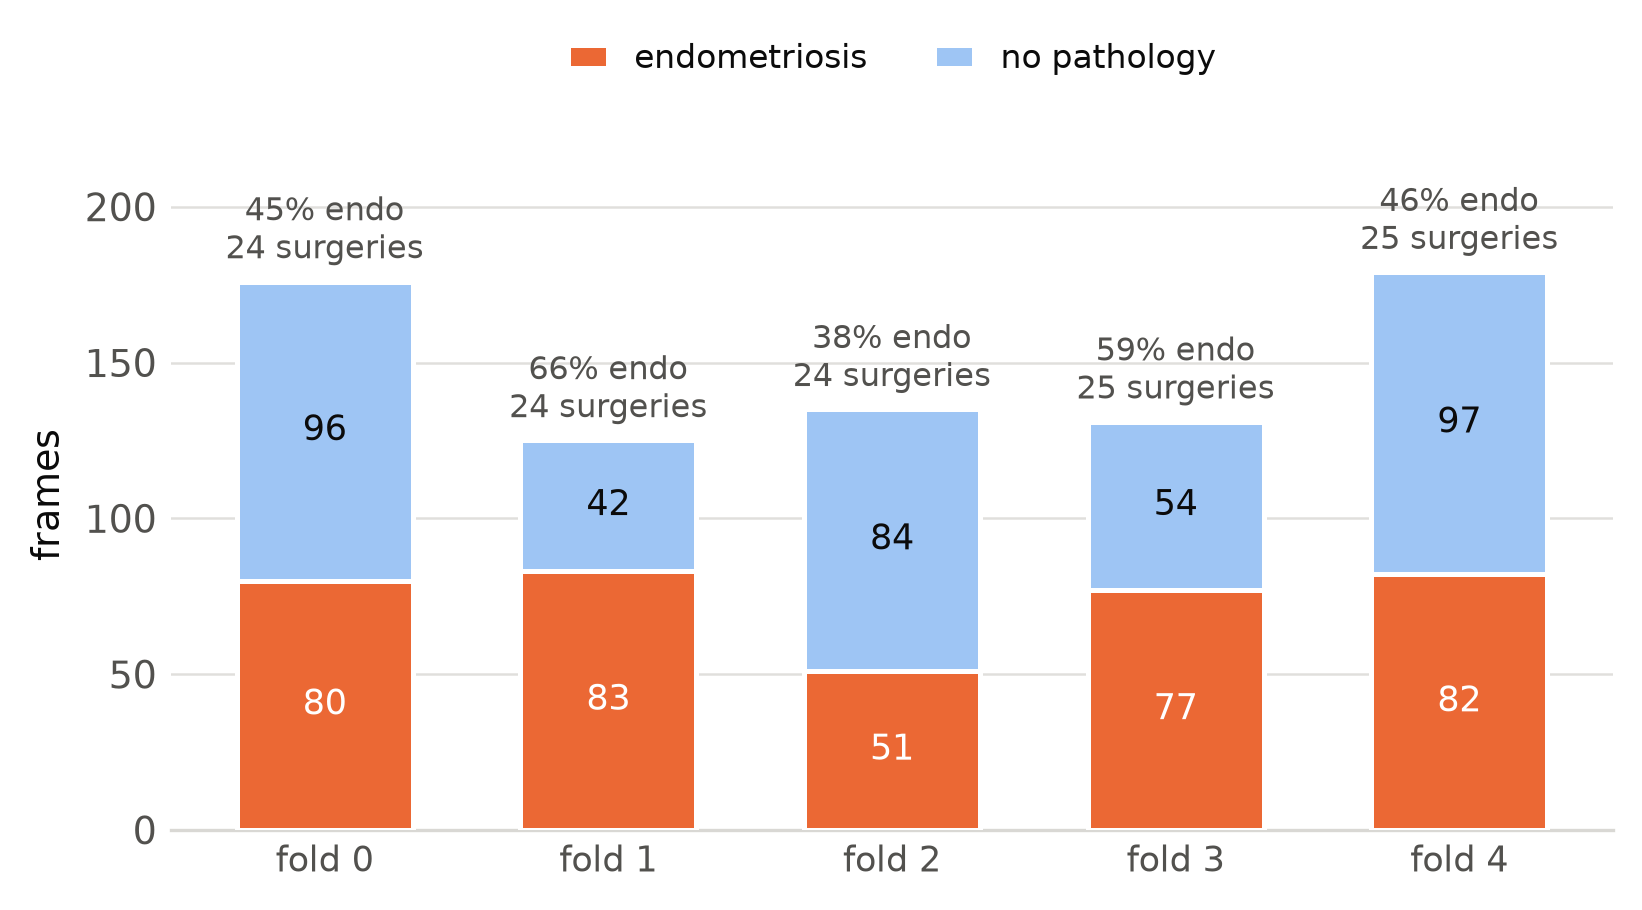
\includegraphics[width=\linewidth]{figures/fig_dataset_folds.png}
\caption{Fold composition. Each bar is one cross-validation fold, split into endometriosis and no-pathology frames, with the pathology share and the number of surgeries above it. Because whole surgeries are kept together, prevalence varies from 37.8\% to 66.4\%, which is why ROC-AUC rather than accuracy is compared across folds.}
\label{fig:folds}
\end{figure}

\begin{figure}[t]
\centering
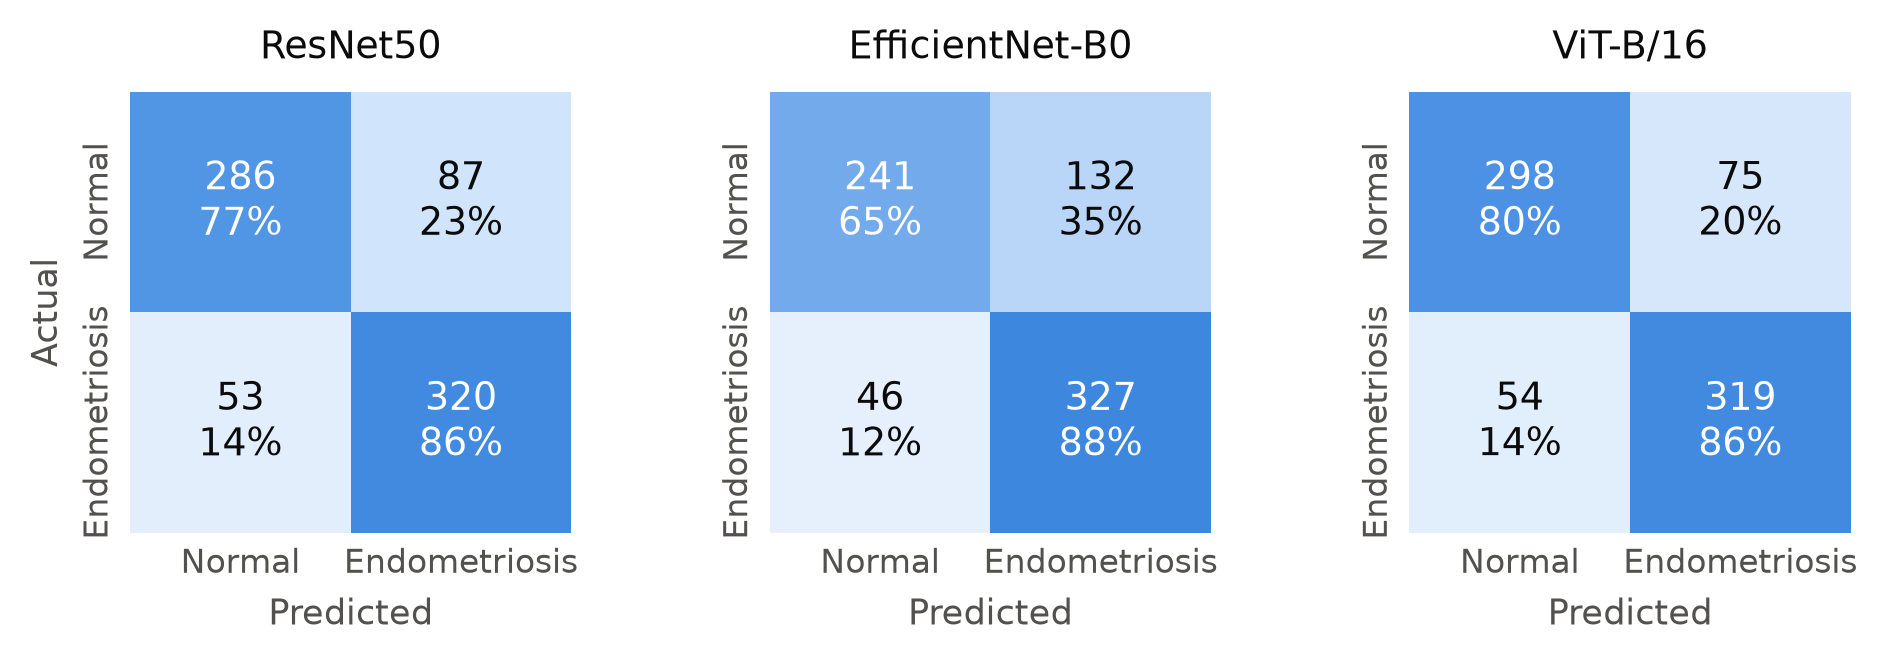
\includegraphics[width=\linewidth]{figures/fig_confusion_pooled.png}
\caption{Pooled out-of-fold confusion matrices over all 746 frames, each predicted by the model that never saw its surgery. Cell shading is the row-normalised share; counts are given inside each cell.}
\label{fig:confusion}
\end{figure}

\begin{figure}[t]
\centering
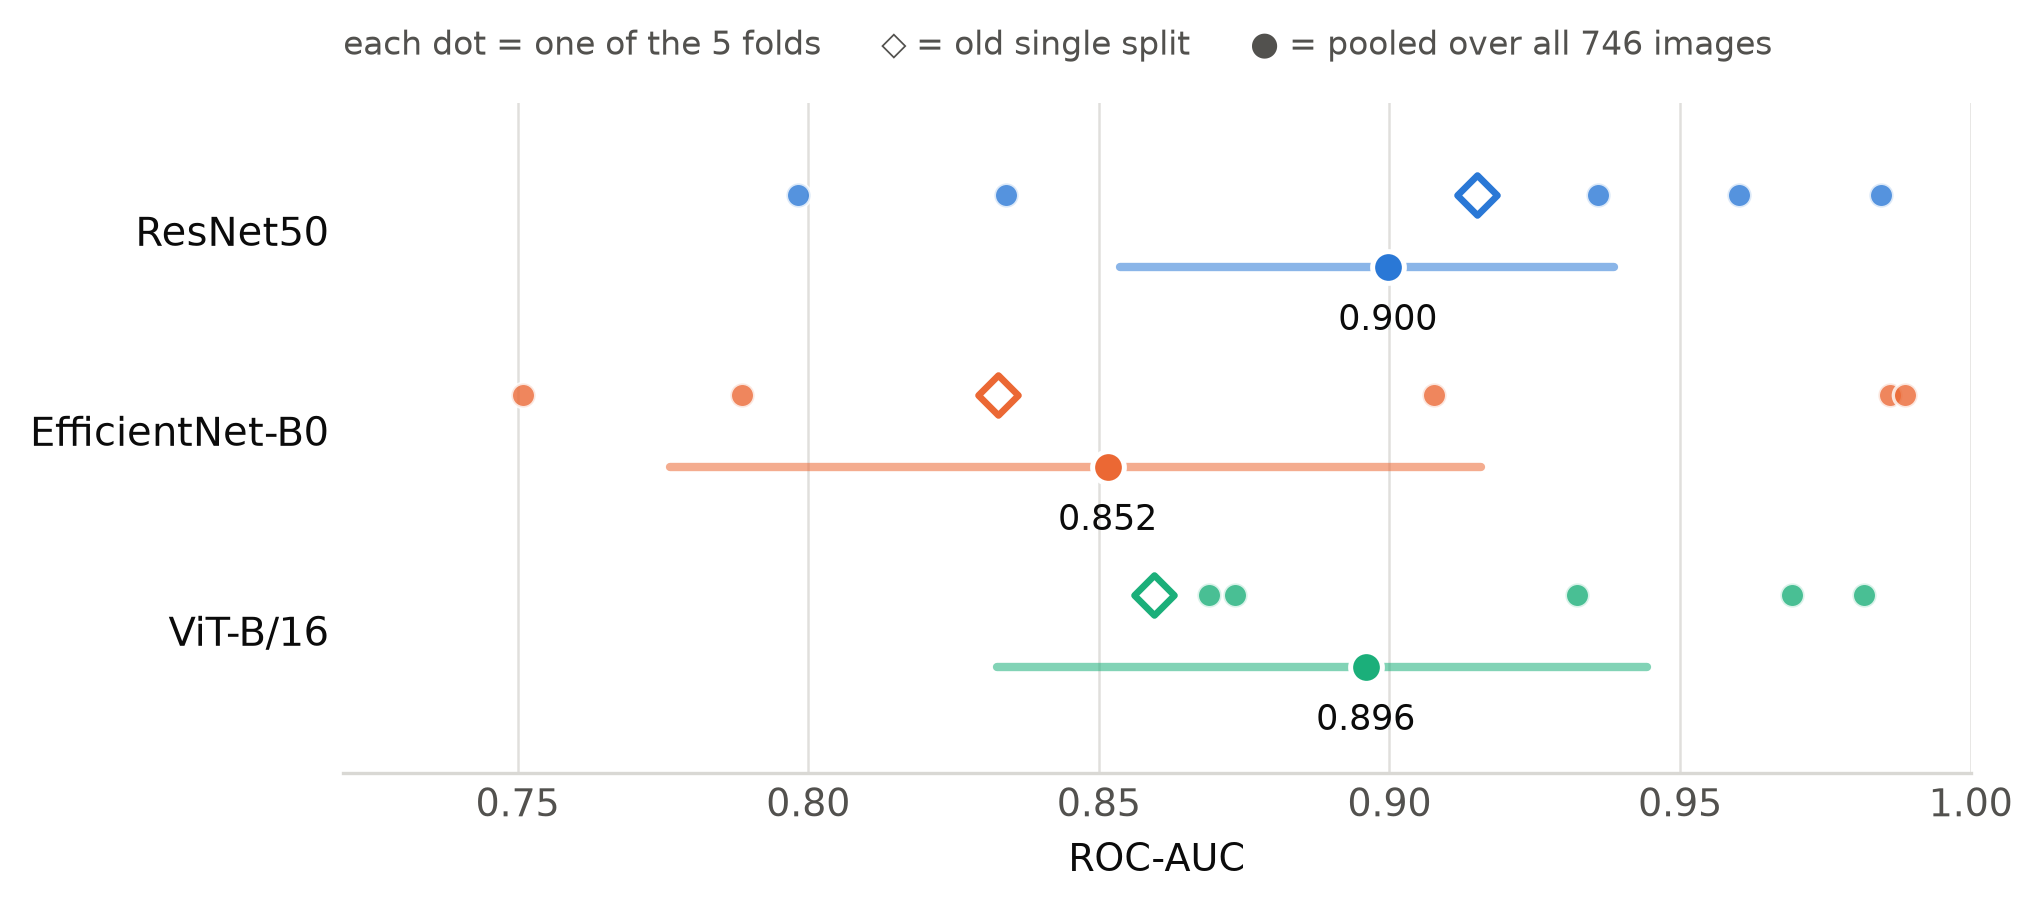
\includegraphics[width=\linewidth]{figures/fig_cv_auc.png}
\caption{Classification performance per architecture. Small dots are the five fold-level AUCs, the open diamond is the earlier single-split estimate, and the filled marker with its bar is the pooled out-of-fold AUC with a 95\% surgery-level bootstrap interval.}
\label{fig:cvauc}
\end{figure}

\begin{figure}[t]
\centering
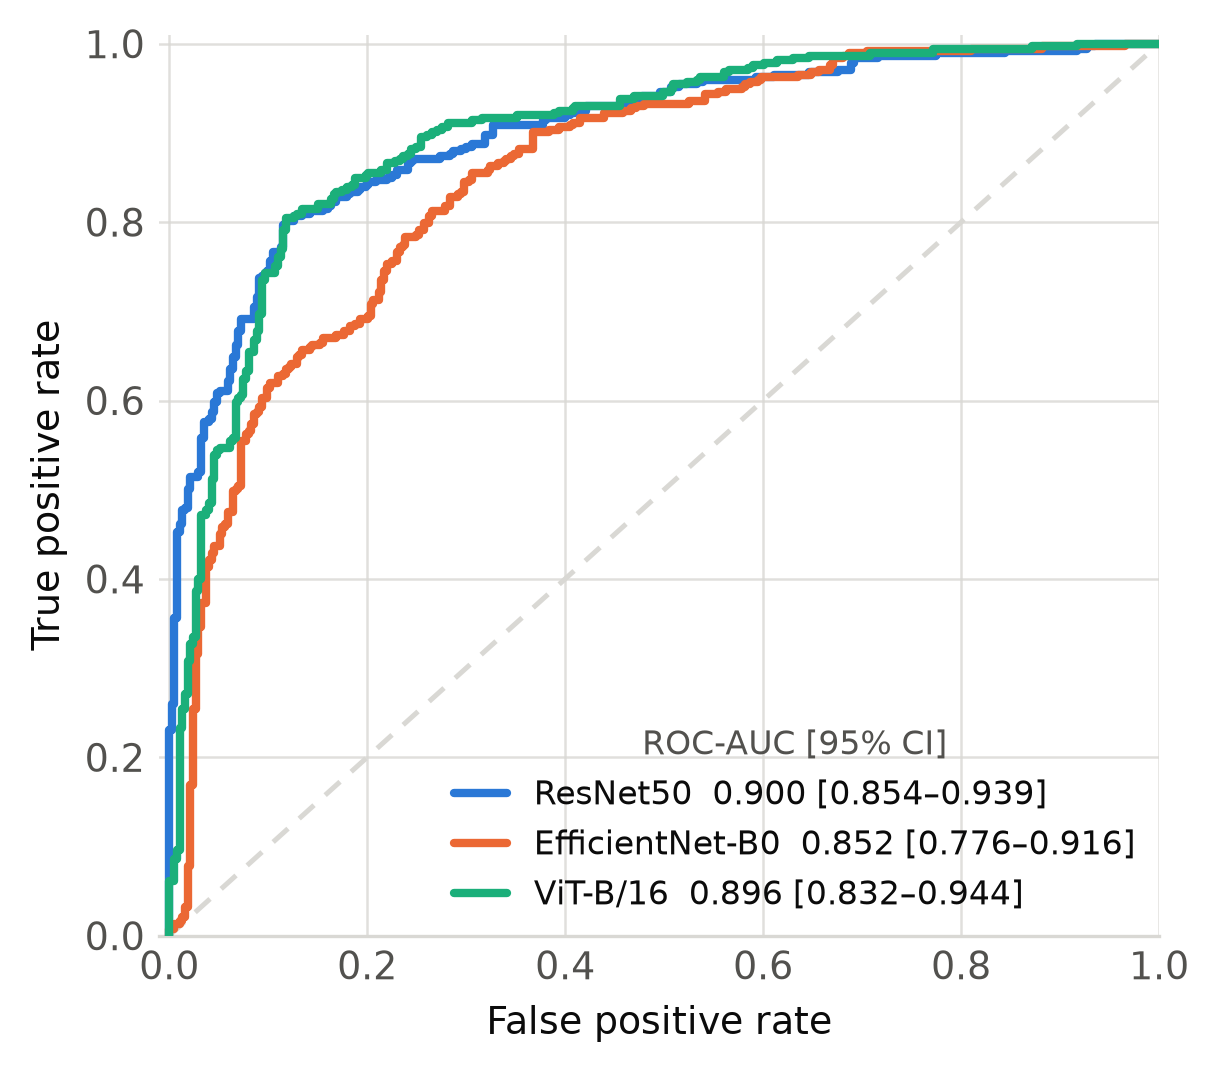
\includegraphics[width=\linewidth]{figures/fig_roc_pooled.png}
\caption{Pooled out-of-fold ROC curves. Each curve aggregates the predictions of the five fold models, so every frame contributes once, scored by a model blind to its surgery. Intervals in the legend resample surgeries.}
\label{fig:roc}
\end{figure}

\begin{figure}[t]
\centering
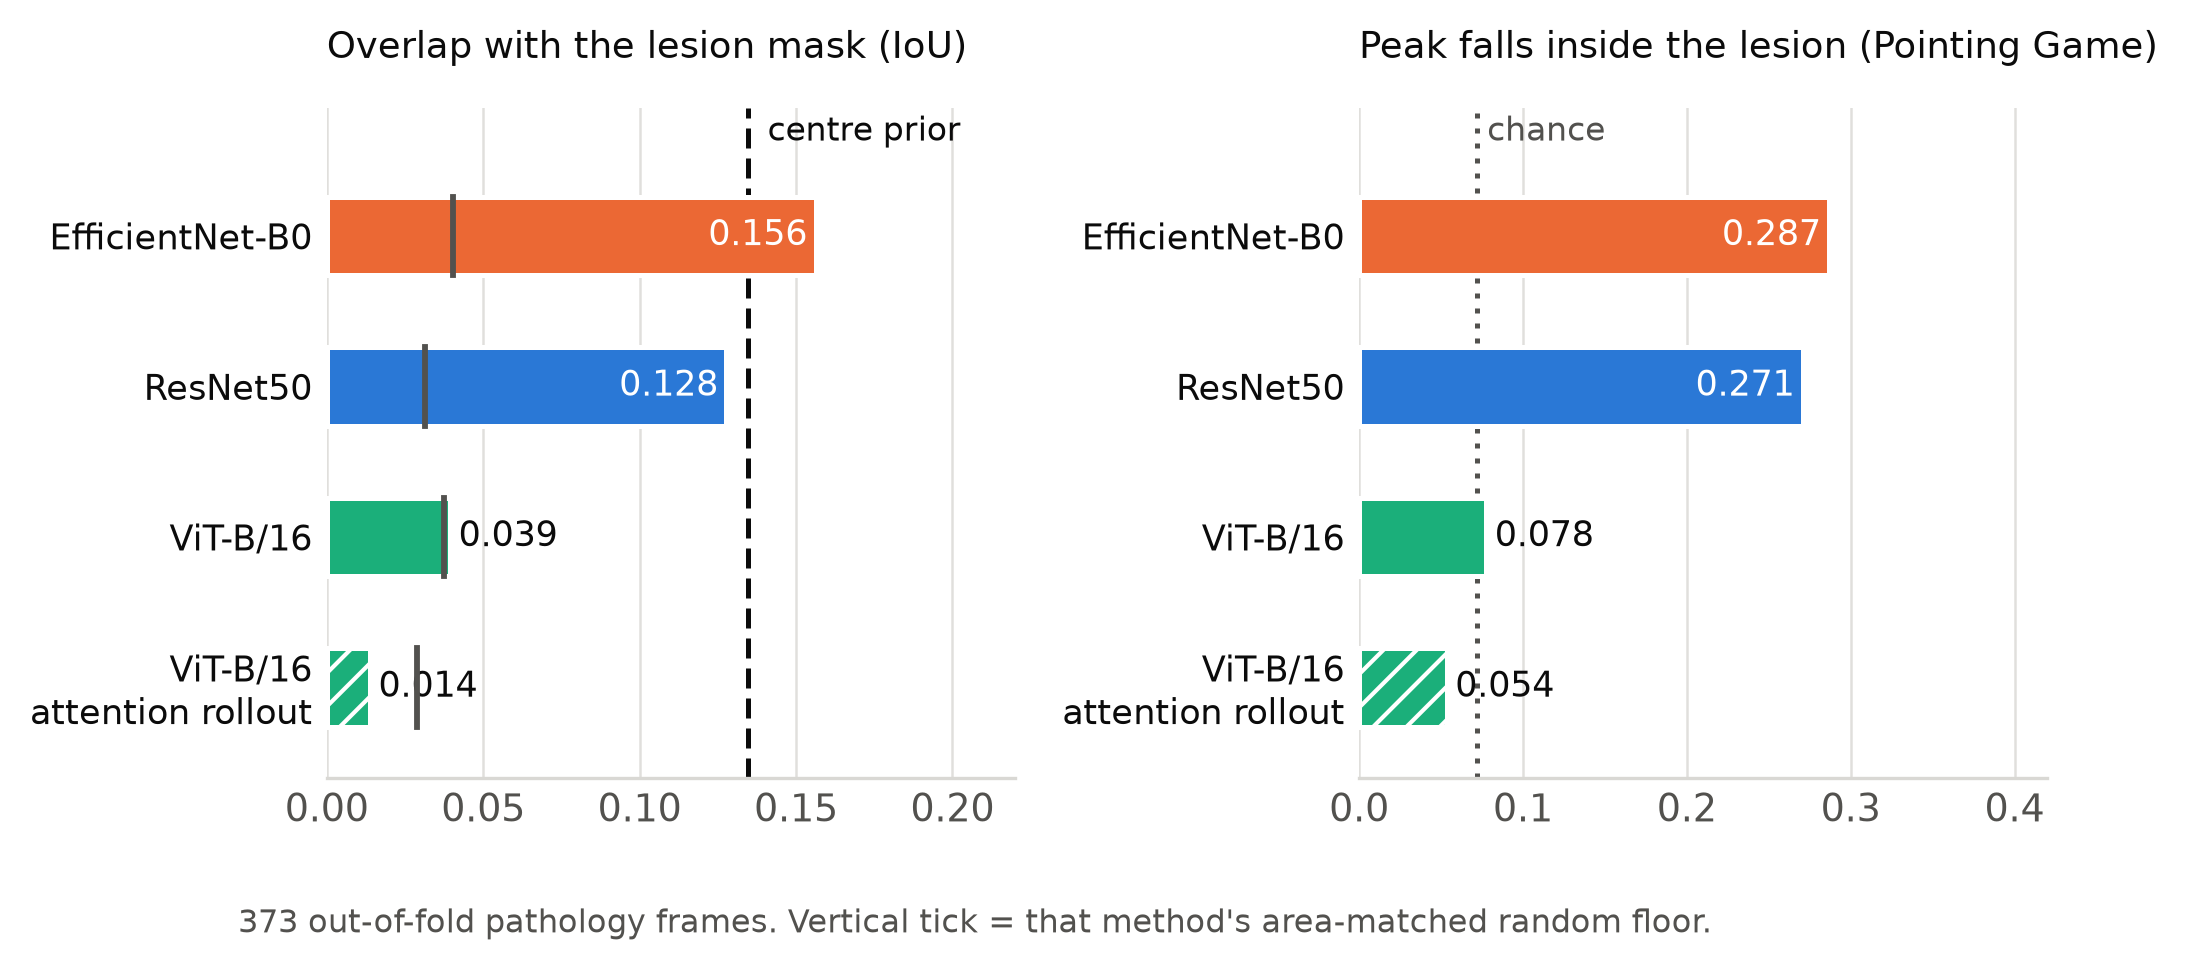
\includegraphics[width=\linewidth]{figures/fig_localization.png}
\caption{Agreement between each saliency map and the expert lesion mask, over all 373 out-of-fold pathology frames. The vertical tick on each bar is that method's own area-matched random floor; the dashed line is a centred Gaussian baseline and the dotted line the chance level for the Pointing Game.}
\label{fig:localization}
\end{figure}

\begin{figure}[t]
\centering
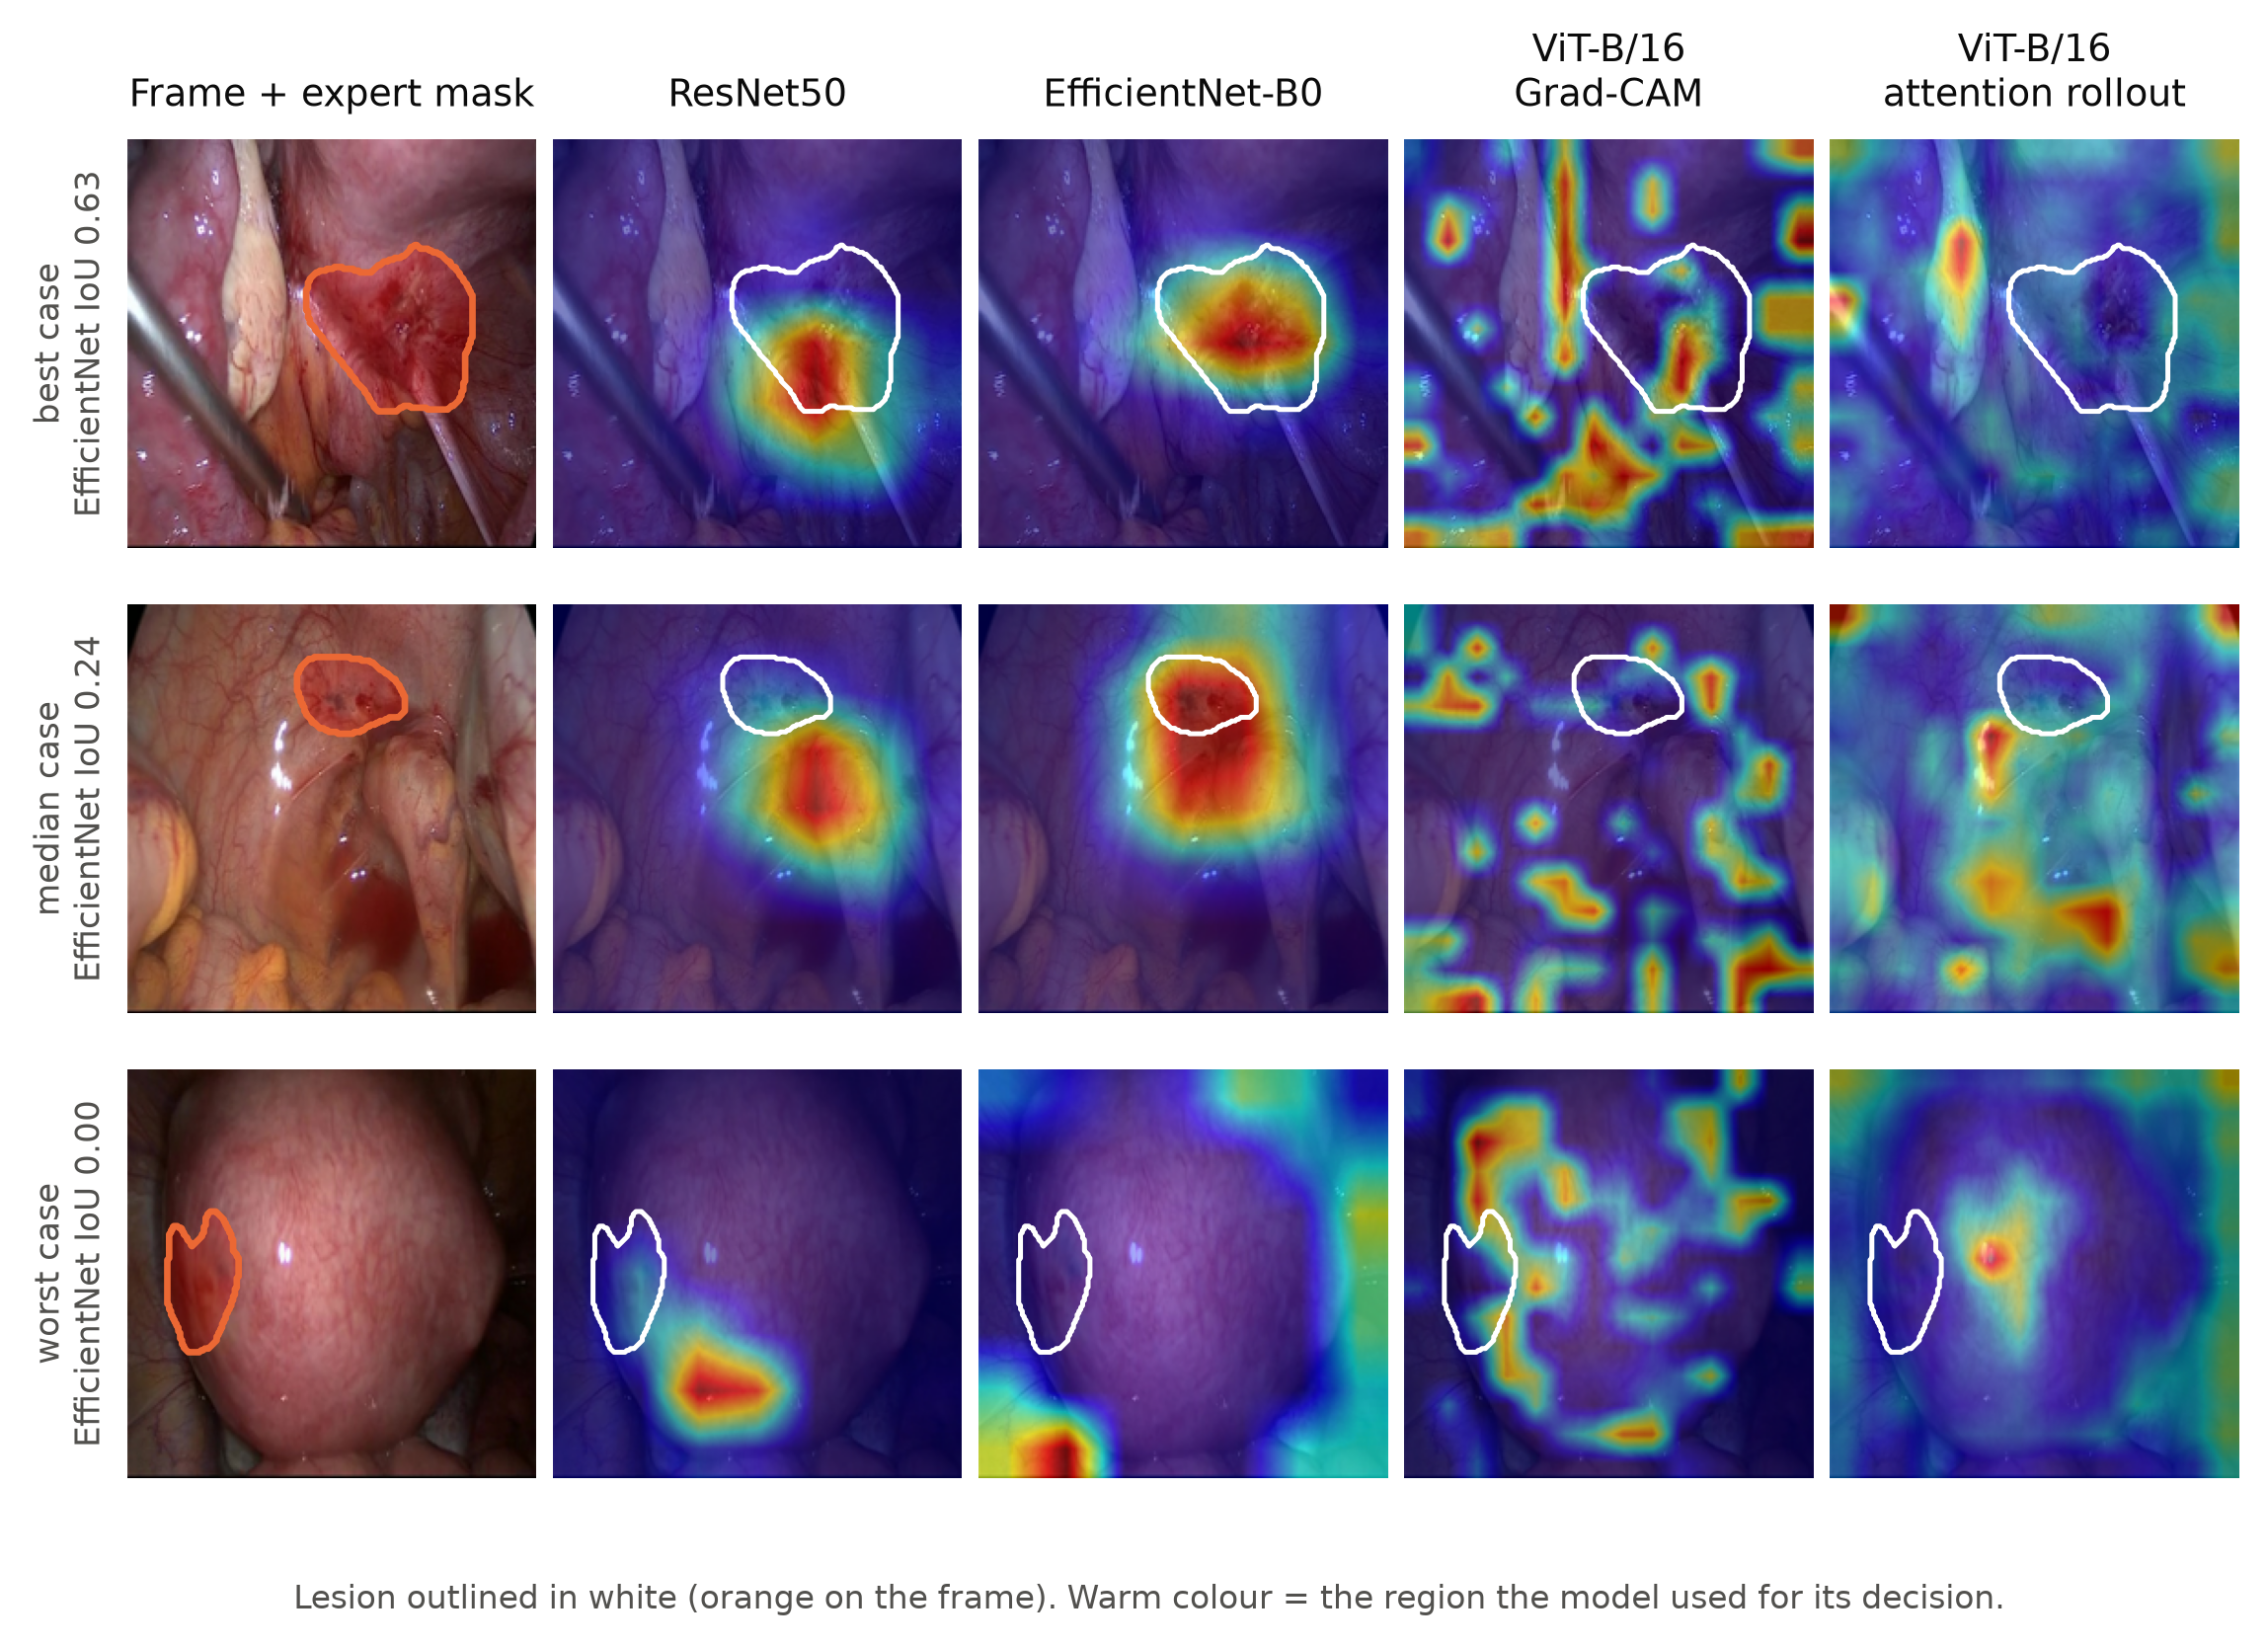
\includegraphics[width=\linewidth]{figures/fig_overlays.png}
\caption{Qualitative comparison on the best, median and worst frames of EfficientNet-B0's IoU distribution. Columns: frame with the expert mask, Grad-CAM for each architecture, and attention rollout for ViT-B/16. Maps shown here come from the preliminary single-split models and are illustrative; all reported numbers use the fold models.}
\label{fig:overlays}
\end{figure}

\begin{figure}[t]
\centering
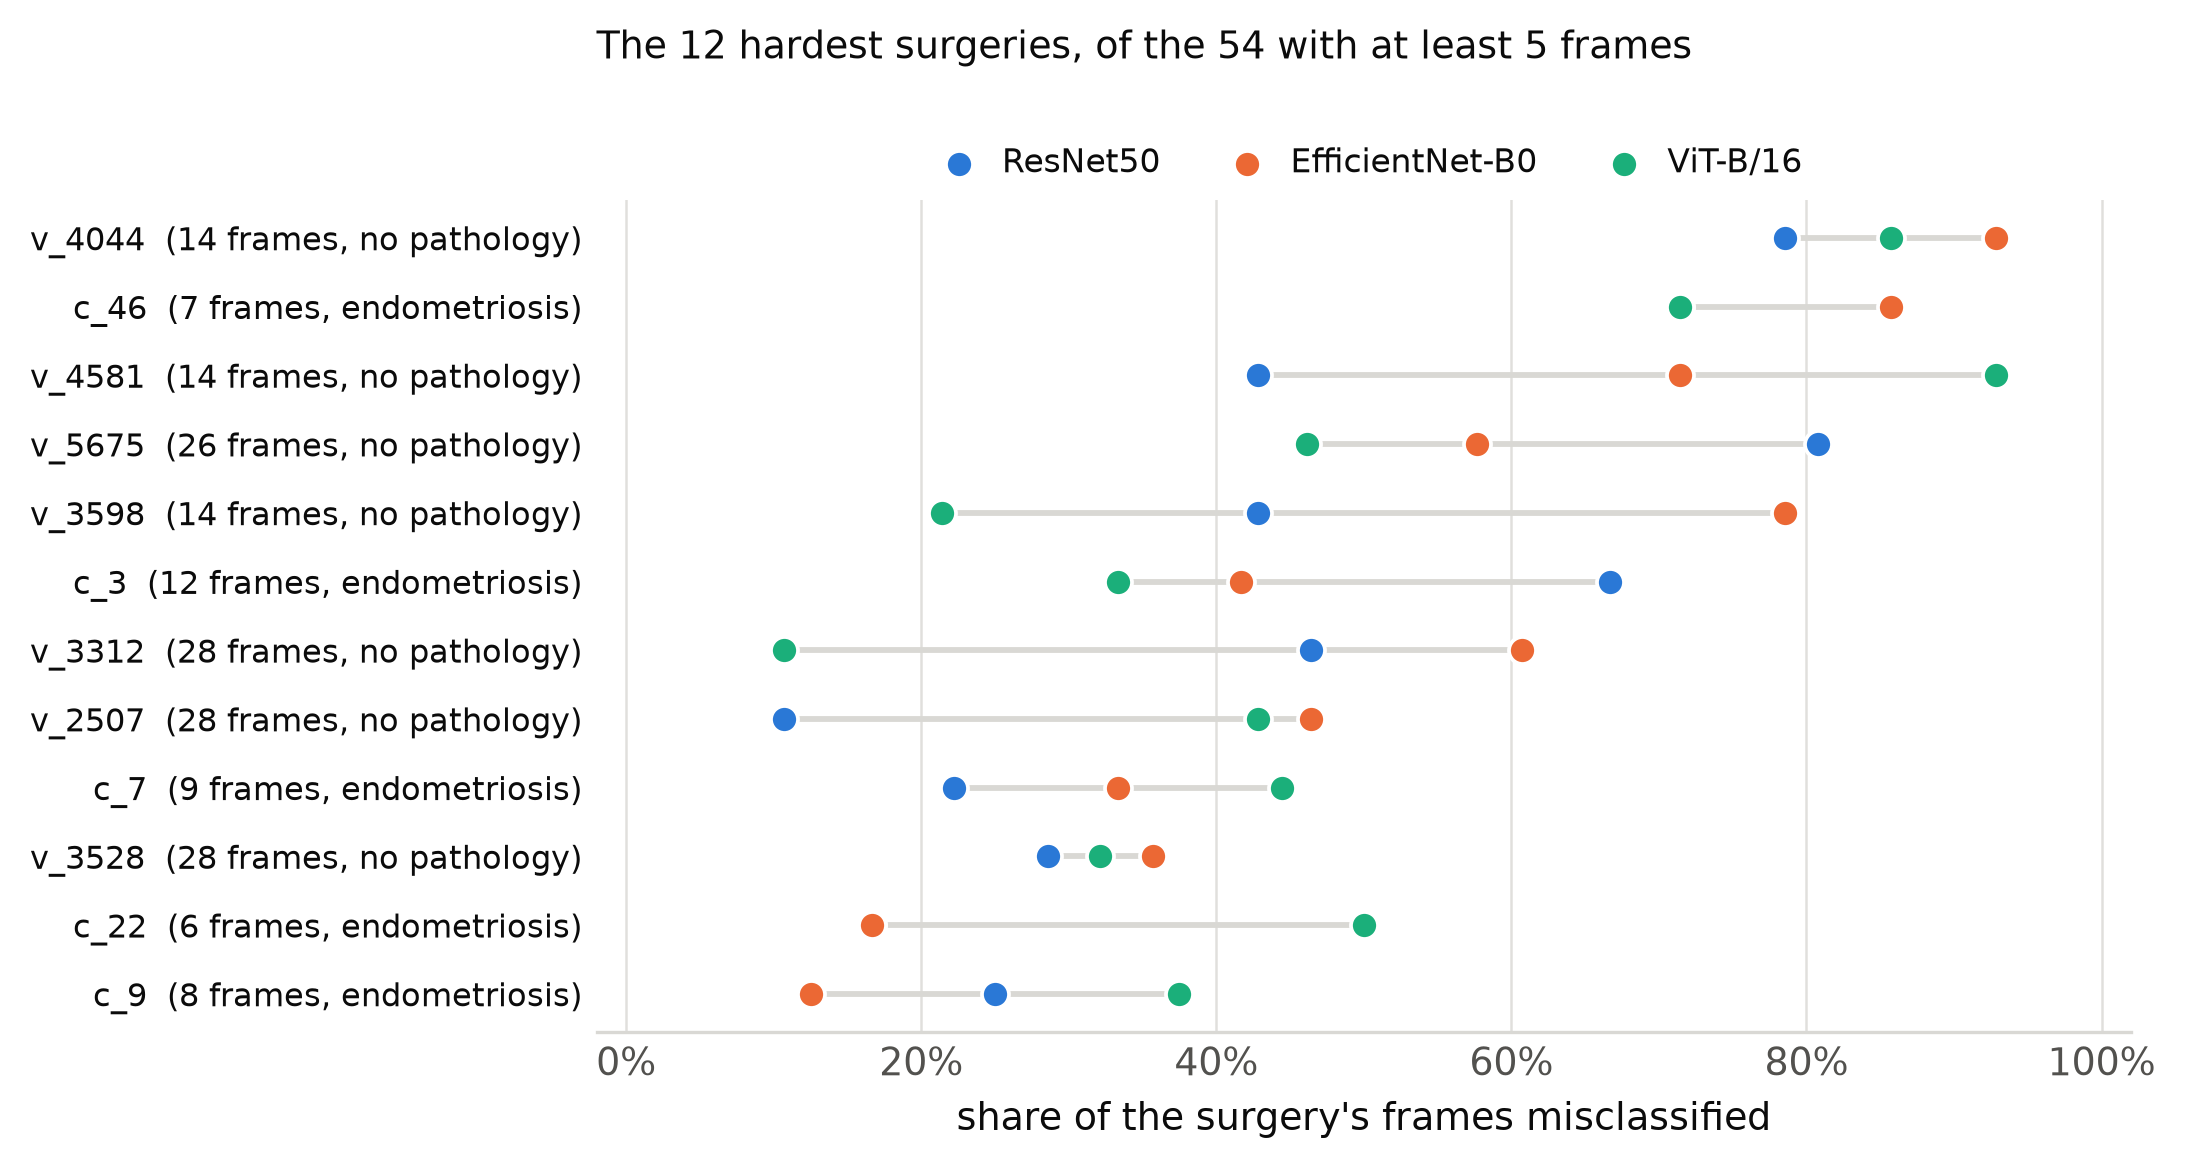
\includegraphics[width=\linewidth]{figures/fig_error_clusters.png}
\caption{Per-surgery error rate for the twelve hardest surgeries among those contributing at least five frames. Errors concentrate in particular recordings rather than spreading across the dataset.}
\label{fig:errors}
\end{figure}

\section{Discussion}
\label{sec:discussion}

\subsection{Two properties that do not travel together}

The central result is a dissociation. The evaluation found no evidence that ViT-B/16 classifies worse than ResNet50, yet ViT-B/16's saliency maps are indistinguishable from chance on all three localization measures. EfficientNet-B0 is the one model this evaluation places below another on AUC, yet it is the only one whose maps exceed a centred-Gaussian baseline on IoU. Ranking by discrimination and ranking by explanation quality do not agree.

This matters because the two are routinely treated as one. A paper that reports a strong AUC and prints a few heat maps invites the reading that the model has learned the lesion. Our measurements show that the inference does not hold here: a model with no detectable disadvantage in discrimination produced maps with no detectable spatial signal.

One hypothesis fits both halves of the dissociation and the error analysis, and we state it as a hypothesis because our experiments do not test it. The errors cluster in particular no-pathology recordings rather than scattering across the dataset, which indicates that recording-level appearance carries information the models can use. A high-capacity model with global receptive fields, such as ViT-B/16, is well placed to exploit that context, and a decision made from context distributed across the frame has no compact region to highlight. EfficientNet-B0, with a sixteenth of the parameters and a convolutional inductive bias, has less room to do so and may be pushed toward local lesion texture --- which would cost a little discrimination while producing maps that fall on the lesion. Testing this would require manipulating the available context, for instance by occluding the lesion region and measuring the performance each architecture retains.

\subsection{What the localization numbers do and do not establish}

IoU, Pointing Game and Coverage measure spatial agreement between a saliency map and an expert mask. They do not measure faithfulness. A map that overlaps the lesion does not prove the model used lesion evidence, and a map that does not overlap it does not prove the model ignored the lesion: the map may simply be a poor summary of the computation. The honest claim is narrower than "EfficientNet-B0 reasons about lesions": its maps agree with expert annotations more than the alternatives do, and ViT-B/16's maps agree no more than chance.

The chance references are what make these numbers interpretable, and we would argue for them as standard practice. Lesions cover 7.2\% of a frame here, so an uninformative map scores 0.072 on two of the three measures by construction, and an IoU figure cannot be read without knowing how much area the method claimed. The centred Gaussian is the more demanding reference and the more revealing one: ResNet50's maps, which look reasonable to the eye and are significantly above random, are statistically indistinguishable from a fixed blob in the middle of the frame. Reported alone, its IoU of 0.128 would have suggested a model that localizes.

Attention rollout deserves a note. It was included to pre-empt the objection that Grad-CAM is unfair to a transformer, and the result is stronger than expected: the transformer-native method performs \emph{worse} than Grad-CAM on ViT-B/16, and falls below the area-matched random floor. Vanilla rollout is class-agnostic --- it aggregates attention flow without reference to the predicted class --- so a diffuse result is consistent with its known behaviour. We therefore do not claim that ViT-B/16 cannot be explained, only that neither of the two standard options produces lesion-aligned maps here. Gradient-weighted transformer attribution remains to be tried.

\subsection{How fragile the comparison is}

Three evaluation protocols on the same data and the same architectures produced two different orderings, and the one that differs is the one with the grouping mistake. A single case-wise split and a cross-validation grouped by recording both rank ResNet50 first and EfficientNet-B0 last; a cross-validation that treated each no-pathology segment folder as a unit puts EfficientNet-B0 first. The effect of that single choice is larger than any difference we can establish between architectures.

Two practical conclusions follow. First, in this dataset a single train/test split did not support a stable ranking, so a study of comparable size that reports one should be read as provisional. Second, the grouping unit must be stated and justified, not assumed: our own segment-level grouping looked rigorous --- it was group-aware cross-validation with assertions --- yet it let four recordings place frames on both sides of a split, which moved EfficientNet-B0's pooled AUC by 0.06. Datasets that ship frames in per-segment folders invite exactly this error.

We would also argue for surgery-level uncertainty as the default in frame-level studies. Resampling frames rather than surgeries narrowed our intervals by a factor of 1.9 to 2.6, which is the difference between reporting two of the three pairwise AUC differences as significant and reporting one. The inference a reader cares about is to new patients, and that is the level at which the data are independent.

\subsection{Error structure and what it implies}

The surgeries with the highest error rates are predominantly no-pathology recordings, and in the worst of them, a single no-pathology recording, every model misclassifies most frames. The failure mode is a systematic false positive on healthy tissue in particular recordings rather than missed lesions --- all three models recall pathology frames at 0.855 to 0.877. Since folds are grouped by surgery, these frames were never trained on, so the clustering reflects something that differs between recordings. We did not measure what: illumination, tissue appearance, instrument presence and camera hardware are all plausible and all confounded in this dataset.

For a screening or second-opinion application this pattern is more actionable than an aggregate error rate. It suggests that performance should be reported per recording rather than pooled, and that the cases to collect next are normal recordings that differ in acquisition, not simply more frames.

\subsection{Clinical reading}

These results do not support clinical use, and we make no such claim. Three limits are decisive. The evaluation set is balanced 1:1 while unselected laparoscopy frames are closer to 1:36, so the precision reported here is an artefact of the evaluation design and would fall substantially at realistic prevalence. We did not assess calibration or decision utility, so the predicted probabilities should not be read as risk estimates. And the task as posed --- a still frame labelled endometriosis or not --- is not the clinical task, in which a surgeon integrates motion, manipulation and tactile feedback across an entire procedure.

What the results do support is narrower and still useful: under cross-validation grouped by surgery, frame-level discrimination between endometriosis and no-pathology laparoscopy frames is feasible with modest data, and recall is the stronger half of the performance profile, which is the direction a screening aid would want.

The explanation findings carry a specific warning for deployment. If a system displays a heat map alongside its prediction, that map is part of the clinical interface, and a map at chance level may not be a neutral addition: it can offer the appearance of a reason where our measurements find none. Whether clinicians' confidence is actually affected is an empirical question we did not study. On this dataset, a ViT-B/16 deployed with Grad-CAM would have produced exactly that. Where explanations are shown to clinicians, their spatial agreement with expert annotation should be measured and reported, not assumed --- and measured against chance, since otherwise plausible-looking numbers can mean nothing.

\section{Limitations and Future Work}
\label{sec:limitations}

\textbf{Scale and statistical power.} The balanced subset contains 746 frames from 122 surgeries, which is what the public data allow. Because the resampling unit is the surgery, the effective sample size for every comparison is of that order, and only one classification difference survived correction. A study of this size can establish that explanation quality differs sharply between architectures; it cannot settle which of them classifies best. Larger multi-centre collections, or federated evaluation across institutions, would be needed for that.

\textbf{Evaluation on a balanced subset.} We rebalanced the data 1:1 so that accuracy and AUC would be informative, but the source distribution is roughly 1:36. The precision reported here is a property of the evaluation design and would fall at realistic prevalence; nothing in this study estimates the positive predictive value a deployed system would have.

\textbf{Task definition.} Frames are labelled only as pathological or not. We do not distinguish lesion type, stage or severity, all of which matter clinically, and we do not use video: a surgeon integrates motion, probing and tactile feedback that a still frame discards. Nor did we assess calibration or decision utility, so the predicted probabilities should not be read as risk estimates.

\textbf{What the explanation metrics measure.} IoU, Pointing Game and Coverage quantify spatial agreement between a saliency map and an expert mask. They do not establish faithfulness: a map that lands on the lesion does not prove the model used lesion evidence, and a map that does not may simply summarise the computation poorly. GLENDA provides one annotation per frame, so we cannot report inter-annotator variability or treat the mask as a range rather than a point. We also fixed the map threshold at 0.5 and used a single target layer per architecture; both choices affect the absolute numbers. The ordering of the two CNNs above both transformer methods is stable across all three metrics, but the two CNNs themselves change places on Coverage (ResNet50 0.168 against EfficientNet-B0 0.153) while IoU and Pointing Game put EfficientNet-B0 first. Only two explanation methods were tested, and the failure of attention rollout does not rule out gradient-weighted transformer attribution performing better.

\textbf{Protocol dependencies.} Pooling out-of-fold predictions assumes the five fold models produce scores on comparable scales; we report the fold-wise summary beside the pooled one rather than verifying that assumption. Learning rates were set per architecture in advance rather than tuned per fold, which keeps the comparison simple but may not place each architecture at its best. Finally, the exact partition depends on the \texttt{StratifiedGroupKFold} implementation: running the same seed under a different scikit-learn version produced different folds, with prevalence ranging differently across them. We release the split manifest and a hash of the frame-to-fold assignment so that the reported numbers can be reproduced, but the folds themselves are not canonical.

\textbf{Directions.} The error analysis points to recording-level appearance as the dominant source of failure, so the most useful next data are no-pathology recordings that differ in acquisition rather than more frames from the same ones. The dissociation we report invites a causal test: occluding the annotated lesion and measuring how much performance each architecture retains would show directly how much of each model's decision rests on the lesion rather than its surroundings.

\section{Conclusion}
\label{sec:conclusion}

We compared ResNet50, EfficientNet-B0 and ViT-B/16 on binary endometriosis classification in laparoscopic frames under a single protocol: a balanced GLENDA subset, 5-fold cross-validation grouped by surgery, and uncertainty estimated by resampling surgeries rather than frames. Alongside classification we measured what each model's saliency map actually covers, scoring Grad-CAM --- and, for the transformer, attention rollout --- against GLENDA's expert lesion masks on every pathology frame, using the fold models that never saw those surgeries.

Three results follow. First, classification did not separate the architectures: after correction, the only difference this evaluation establishes is that ResNet50 discriminates better than EfficientNet-B0 ($\Delta$AUC +0.048, \emph{p} = 0.030), and the ordering of the three models reversed when the grouping unit was set to the segment rather than the recording. Second, explanation quality did separate them, decisively and in the opposite direction: EfficientNet-B0 is the only model whose maps exceed a centre-of-image baseline on IoU, ResNet50's are indistinguishable from that baseline, and ViT-B/16's are indistinguishable from chance on all three measures --- a result attention rollout does not repair. Third, the two properties therefore do not order the architectures the same way, so a model chosen on AUC alone may be the one whose explanations carry least information.

For practice, two things follow. Where a system displays a saliency map alongside its prediction, that map should be measured against the annotation and against chance, not displayed on the assumption that a good classifier explains well. And where frames come from recordings, the grouping unit should be stated and justified: setting it one level too fine was enough, in our data, to change which architecture appeared best.

The study is limited by scale --- 122 surgeries --- by its balanced evaluation set, and by the fact that spatial agreement with a mask is not faithfulness. Establishing why the dissociation arises will need an intervention rather than an observation; occluding the annotated lesion and measuring what performance each architecture retains is the most direct test we can suggest.

\bibliographystyle{elsarticle-num}
\bibliography{references}
\end{document}
